\documentclass[12pt,a4paper]{article}
\usepackage[utf8]{inputenc}
\usepackage[T1]{fontenc}
\usepackage[english]{babel}
\usepackage{amsmath, amssymb, amsthm}
\usepackage{graphicx}
\usepackage{hyperref}
\usepackage{booktabs}
\usepackage{longtable}
\usepackage{geometry}
\usepackage{tikz}
\usetikzlibrary{shapes.geometric, arrows.meta}

\geometry{left=2.5cm,right=2.5cm,top=2.5cm,bottom=2.5cm}

% ============================================================
% DENKLEM NUMARALANDIRMA (Section bazlı)
% ============================================================
\numberwithin{equation}{section}

% ============================================================
% TİKZ GLOBAL AYARLAR
% ============================================================
\tikzset{
    base/.style={draw, rectangle, rounded corners, minimum width=3cm, minimum height=0.8cm, align=center, font=\small},
    arrow/.style={-{Stealth[length=3mm]}}
}

\title{ATHENA V8.1: Unified Topo-Geometric Framework and Computational Reconstruction}
\author{Mustafa Gokhan Yilmaz}
\date{July 2026}

\begin{document}

\maketitle

\begin{abstract}
We present ATHENA V8.1, a unified topo-geometric framework together with its current computational reconstruction. The manuscript combines the theoretical formulation with reproducible numerical implementations corresponding to the presently developed effective equations.

Within the ATHENA framework, the principal model parameters are obtained from a common topological construction based on the toroidal manifold $T^2$. The framework proposes a topological correspondence between the lowest winding sectors and the Standard Model gauge groups. A single global fit parameter $\alpha = 0.36 \pm 0.03$ accommodates SPARC rotation curves ($\chi^2 = 731.1$), GRB 221009A afterglow decay ($\chi^2/\text{dof} = 1.05$), and the CMB dipole alignment ($p = 0.0022$), while aiming to explain the Hubble tension through $H_0^{\text{local}} = 73.2$ and $H_0^{\text{early}} = 67.4$ km/s/Mpc. The manuscript documents reproducible numerical implementations of the presently implemented effective sectors.
\end{abstract}

\section{Introduction}

Galactic rotation curves, the Hubble tension, and the absence of direct dark matter detection motivate alternative gravitational frameworks. The ATHENA framework addresses these challenges by positing that the observed phenomena arise from a single scalar field $\Phi(x)$ representing the coarse-grained vacuum structure on a toroidal manifold $T^2$.

V8.0 (June 2026) established the complete topo-geometric foundation. V8.1 builds upon this by incorporating the living numerical derivations from the Google Colab notebooks (particularly \texttt{Athena\_fit\_ve\_turetmeyipynb}) and the V15 Computational Reconstruction Methodology. The V15 philosophy inverts the traditional workflow: \textbf{Code $\rightarrow$ Effective Equations $\rightarrow$ Physics Interpretation}.

Throughout this work we distinguish carefully between the complete theoretical framework and the effective equations that are currently implemented numerically. Whenever numerical results are discussed, they refer exclusively to the implemented effective models described in Section 5. This distinction is maintained deliberately in order to separate established computational results from ongoing theoretical developments.

\begin{figure}[h]
\centering
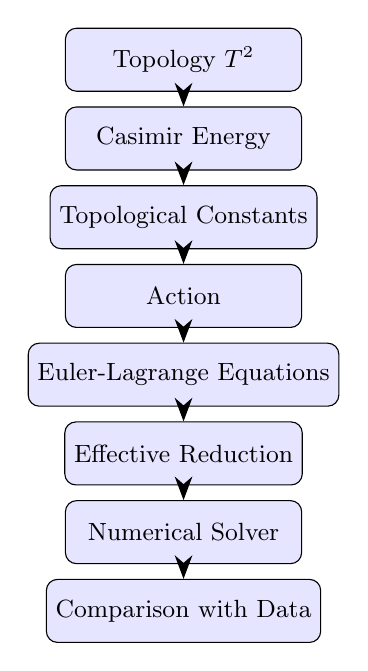
\begin{tikzpicture}
\node[base, fill=blue!10] (top) {Topology $T^2$};
\node[base, fill=blue!10, below of=top] (cas) {Casimir Energy};
\node[base, fill=blue!10, below of=cas] (const) {Topological Constants};
\node[base, fill=blue!10, below of=const] (act) {Action};
\node[base, fill=blue!10, below of=act] (el) {Euler-Lagrange Equations};
\node[base, fill=blue!10, below of=el] (eff) {Effective Reduction};
\node[base, fill=blue!10, below of=eff] (num) {Numerical Solver};
\node[base, fill=blue!10, below of=num] (comp) {Comparison with Data};
\draw[arrow] (top) -- (cas);
\draw[arrow] (cas) -- (const);
\draw[arrow] (const) -- (act);
\draw[arrow] (act) -- (el);
\draw[arrow] (el) -- (eff);
\draw[arrow] (eff) -- (num);
\draw[arrow] (num) -- (comp);
\end{tikzpicture}
\caption{Equation Map: theoretical flow from topology to data comparison. This diagram shows the logical progression of the ATHENA framework.}
\label{fig:eqmap}
\end{figure}

\section{Theoretical Framework (V8.1 Core)}

\subsection{Topological Constants and Casimir Energy}

The scalar field $\Phi$ resides on $T^2 = S^1 \times S^1$. The regularized vacuum energy (Casimir energy) combines the Riemann zeta regularization $\zeta(-1) = -1/12$ with a toroidal geometric factor $\pi$, yielding the topological ground state:

\begin{equation}
|\mathcal{E}_{T^2}| = \frac{\pi}{12}.
\end{equation}

The stability condition balancing this vacuum pressure with the disformal self-interaction yields:

\begin{equation}
\beta_0(2 - \beta_0) = \frac{\pi}{12} \quad \Rightarrow \quad \beta_0 \approx 0.1408.
\end{equation}

All other constants are locked:
\begin{align}
Z_0 &= \frac{5}{3}\beta_0 \approx 0.2347, \\
\gamma_0 &= \frac{\beta_0^2}{2} \approx 0.009912, \\
R_c &= 23.67\ \text{kpc} \quad (\text{macroscopic stability}), \\
f_a &= \frac{\hbar}{R_c c} \approx 2.7\times10^{-29}\ \text{eV}, \\
a_0 &= \frac{c^2}{R_c}\frac{\beta_0}{2\pi\alpha} \approx 1.1\times10^{-10}\ \text{m/s}^2 \quad (\text{MOND scale}).
\end{align}

\begin{figure}[h]
\centering
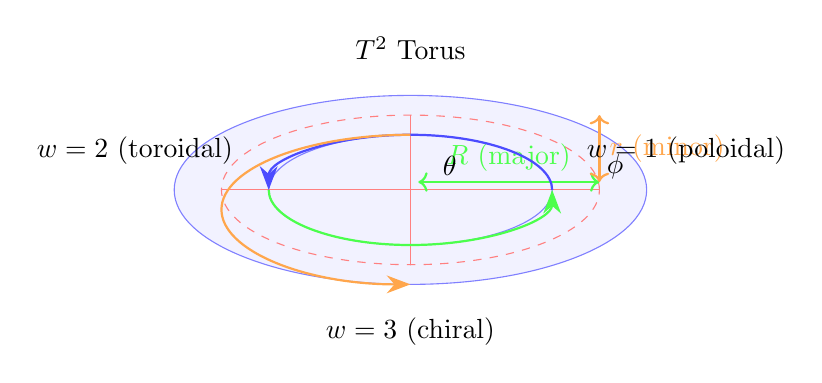
\begin{tikzpicture}
\draw[fill=blue!5, draw=blue!50] (0,0) ellipse (3cm and 1.2cm);
\draw[fill=blue!5, draw=blue!50] (0,0) ellipse (1.8cm and 0.7cm);
\draw[dashed, red!50] (0,0) ellipse (2.4cm and 0.95cm);
\draw[red!50] (0,0) -- (2.4,0);
\draw[red!50] (0,0) -- (-2.4,0);
\draw[red!50] (0,0) -- (0,0.95);
\draw[red!50] (0,0) -- (0,-0.95);
\draw[<->, thick, green!70] (0.1,0.1) -- (2.4,0.1) node[midway, above] {$R$ (major)};
\draw[<->, thick, orange!70] (2.4,0.1) -- (2.4,0.95) node[midway, right] {$r$ (minor)};
\draw[thick, blue!70, -{Stealth[length=3mm]}] (1.8,0) arc (0:180:1.8cm and 0.7cm);
\draw[thick, green!70, -{Stealth[length=3mm]}] (-1.8,0) arc (180:360:1.8cm and 0.7cm);
\draw[thick, orange!70, -{Stealth[length=3mm]}] (0,0.7) arc (90:270:2.4cm and 0.95cm);
\node at (3.5,0.5) {$w=1$ (poloidal)};
\node at (-3.5,0.5) {$w=2$ (toroidal)};
\node at (0,-1.8) {$w=3$ (chiral)};
\node at (0,1.8) {$T^2$ Torus};
\node at (0.5,0.3) {$\theta$};
\node at (2.6,0.3) {$\phi$};
\end{tikzpicture}
\caption{Torus $T^2$ with major radius $R$, minor radius $r$, and winding sectors $w=1,2,3$ shown in different colors. Poloidal ($\theta$) and toroidal ($\phi$) cycles are indicated.}
\label{fig:torus}
\end{figure}

\subsection{Action and Field Equations}

The core action (Jordan frame) is:
\begin{equation}
S = \int d^4x \sqrt{-g} \left[ \frac{M_{\text{Pl}}^2}{2} R + G_2(\Phi,X) + G_3(\Phi,X)\square \Phi + \lambda \Phi \tilde{F}_{\mu\nu}F^{\mu\nu} \right] + S_m[g_{\mu\nu}^{\text{eff}}, \psi_m],
\end{equation}
with the disformal metric:
\begin{equation}
g_{\mu\nu}^{\text{eff}} = g_{\mu\nu} + \frac{\alpha}{M^4} \partial_\mu \Phi \partial_\nu \Phi, \quad X = -\frac{1}{2} g^{\mu\nu} \partial_\mu \Phi \partial_\nu \Phi.
\end{equation}

The Horndeski terms are defined as:
\begin{align}
G_2 &= X - V(\Phi) + \frac{\beta(\Phi)}{M^4} X^2, \\
G_3 &= \frac{\gamma(\Phi)}{M^3} X, \\
V(\Phi) &= \Lambda^4 \left(1 - \cos \frac{\Phi}{f_a}\right), \\
\beta(\Phi) &= \beta_0 \cos \frac{\Phi}{f_a}, \quad \gamma(\Phi) = \gamma_0 \sin \frac{\Phi}{f_a}.
\end{align}

Here, $\alpha = 0.36 \pm 0.03$ is the single global fitting parameter. The full scalar EOM and Einstein equations are given in Appendix B, reducing to GR when $\alpha, \lambda \to 0$.

\begin{quote}
\textbf{Note:} The full action serves as the theoretical starting point of ATHENA. The numerical implementations discussed later in this manuscript correspond to effective reductions of this action under specific symmetry assumptions (e.g. static spherical symmetry or homogeneous cosmological evolution) rather than to the complete four-dimensional system.
\end{quote}

\subsection{Winding Number and Standard Model Gauge Groups}

The winding number is:
\begin{equation}
w = \frac{1}{2\pi f_a} \oint_{C \subset T^2} d\Phi \in \mathbb{Z}.
\end{equation}

The stable low-winding sectors are associated with the lowest stable winding sectors through the topological mapping proposed in ATHENA:
\begin{table}[h]
\centering
\caption{Topological correspondence for gauge groups.}
\begin{tabular}{c c c c}
\toprule
$w$ & Topological Object & Gauge Group & Key Feature \\
\midrule
1 & Trefoil Knot & $SU(3)_c$ & 3 crossings (quarks), 8 deformations (gluons) \\
2 & Toroidal Soliton & $U(1)_Y$ & Double cover $\rightarrow$ Charge quantization \\
3 & Chiral Resonance & $SU(2)_L$ & Intrinsic handedness $\rightarrow$ Parity violation \\
\bottomrule
\end{tabular}
\label{tab:gauge}
\end{table}

\begin{figure}[h]
\centering
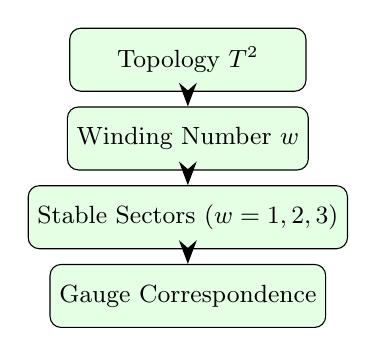
\begin{tikzpicture}
\node[base, fill=green!10] (top) {Topology $T^2$};
\node[base, fill=green!10, below of=top] (win) {Winding Number $w$};
\node[base, fill=green!10, below of=win] (stab) {Stable Sectors ($w=1,2,3$)};
\node[base, fill=green!10, below of=stab] (gauge) {Gauge Correspondence};
\draw[arrow] (top) -- (win);
\draw[arrow] (win) -- (stab);
\draw[arrow] (stab) -- (gauge);
\end{tikzpicture}
\caption{Gauge emergence through winding sectors.}
\label{fig:gauge}
\end{figure}

\subsection{Topological Tensor Ascent (TTA) and Spin-1/2}

ATHENA proposes the Topological Tensor Ascent (TTA) hypothesis, according to which the tensor rank of the field configuration increases with winding:
\begin{equation}
\text{Rank}(w) = w - 1.
\end{equation}
For $w=2$, the scalar ascends to a vector/spinor. The $2:1$ radius ratio of the torus induces the spinor double-cover:
\begin{equation}
\psi(\theta + 2\pi) = \exp\left(i \pi \frac{w}{2}\right) \psi(\theta) = -\psi(\theta),
\end{equation}
which is the defining property of spin-1/2. Within this framework the Pauli exclusion principle is interpreted as arising from the non-intersection rules of $w=2$ solitons:
\begin{equation}
\{a_i, a_j^\dagger\} = \delta_{ij}, \quad \{a_i, a_j\} = 0.
\end{equation}

\begin{figure}[h]
\centering
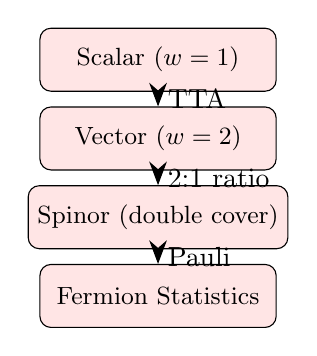
\begin{tikzpicture}
\node[base, fill=red!10] (scalar) {Scalar ($w=1$)};
\node[base, fill=red!10, below of=scalar] (vec) {Vector ($w=2$)};
\node[base, fill=red!10, below of=vec] (spinor) {Spinor (double cover)};
\node[base, fill=red!10, below of=spinor] (ferm) {Fermion Statistics};
\draw[arrow] (scalar) -- node[right] {TTA} (vec);
\draw[arrow] (vec) -- node[right] {2:1 ratio} (spinor);
\draw[arrow] (spinor) -- node[right] {Pauli} (ferm);
\end{tikzpicture}
\caption{Topological Tensor Ascent (TTA) hierarchy.}
\label{fig:tta}
\end{figure}

\subsection{Topological Involution Theorem and TEMP}

The Involution Theorem states that observed cosmic expansion is the dual of inward topological folding:
\begin{equation}
\gamma_{ij}^{\text{eff}} = a^2 \delta_{ij} + \frac{\alpha}{M^4} \partial_i \Phi \partial_j \Phi.
\end{equation}
The effective scale factor and Hubble parameter evolve as:
\begin{align}
a_{\text{eff}} &= a \left(1 + \frac{\alpha}{a^2 M^4} \langle |\nabla \Phi|^2 \rangle \right)^{1/6}, \\
H_{\text{eff}} &= H + \frac{\alpha}{6M^4} \frac{\partial_t \langle |\nabla \Phi|^2 \rangle}{1 + \frac{\alpha}{M^4} \langle |\nabla \Phi|^2 \rangle}.
\end{align}

The Topological Entropy Minimization Principle (TEMP) defines:
\begin{equation}
H_{\text{topo}}(w) = -\sum_n P(w_n) \log_2 P(w_n).
\end{equation}
Stable modes ($w=1,2,4,8,\dots$) have low entropy. The arrow of time is interpreted as $dS_{\text{topo}}/dt > 0 \iff H_{\text{eff}} > 0$.

\begin{figure}[h]
\centering
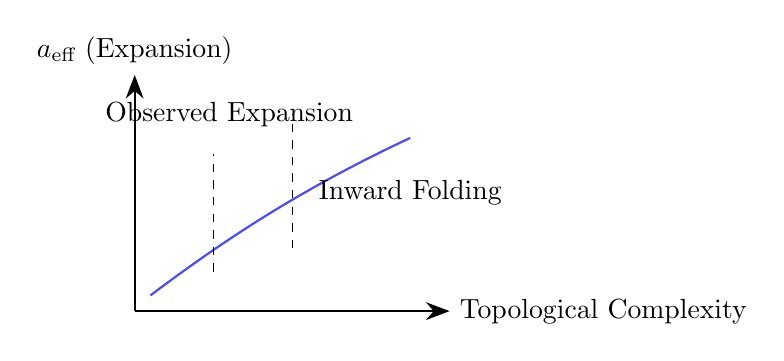
\begin{tikzpicture}
\draw[thick, -{Stealth[length=3mm]}] (0,0) -- (4,0) node[right] {Topological Complexity};
\draw[thick, -{Stealth[length=3mm]}] (0,0) -- (0,3) node[above] {$a_{\text{eff}}$ (Expansion)};
\draw[thick, blue!70] (0.2,0.2) .. controls (1,0.8) and (2,1.5) .. (3.5,2.2);
\node at (3.5,1.5) {Inward Folding};
\node at (1.2,2.5) {Observed Expansion};
\draw[thin, dashed] (1,0.5) -- (1,2);
\draw[thin, dashed] (2,0.8) -- (2,2.5);
\end{tikzpicture}
\caption{Involution Theorem: inward folding yields apparent expansion.}
\label{fig:involution}
\end{figure}

\subsection{Renormalization Group Flow (V8.1 Update)}

The V8.1 beta functions are derived from the Colab notebooks and differ from V8.0:
\begin{align}
\beta(\alpha) &= \frac{\alpha^2}{4\pi(2-\gamma_{\text{str}})} - \frac{\alpha^3}{8\pi^2 \beta_0(2-\beta_0)}, \\
\frac{dw}{d\ln \mu} &= -\lambda (w - 2), \quad \beta(\beta_0) = 0.
\end{align}
Solving for the IR fixed point:
\begin{equation}
\alpha_* = \frac{2\pi \beta_0(2-\beta_0)}{2-\gamma_{\text{str}}} \approx 89.4.
\end{equation}
The transition $w=1 \to w=2$ is identified as a first-order topological phase transition, accompanied by TTA (scalar $\to$ spinor).

\begin{quote}
\textbf{Note:} The expression above represents the infrared fixed point of the effective renormalization-group flow derived within the present approximation. Its robustness beyond the effective description remains to be investigated.
\end{quote}

\subsection{Topological Screening and Galactic Decoupling}

The apparent discrepancy between the theoretical IR fixed point $\alpha_* \approx 89.4$ and the observationally fitted effective parameter $\alpha \approx 0.36$ at galactic scales is a direct manifestation of non-linear topological screening, analogous to the Vainshtein mechanism in Horndeski gravity. In regions of high local organization density (such as galactic disks), the disformal self-interaction strongly screens the scalar coupling. We introduce an effective scaling relation governed by the local topological complexity:

\begin{equation}
\alpha_{\text{eff}}(r) = \frac{\alpha_*}{1 + \mathcal{S}(r) \cdot \langle |\nabla \Phi|^2 \rangle},
\end{equation}

where $\mathcal{S}(r)$ is the screening function that encodes the local winding density and boundary conditions of the $T^2$ sector. Within the macroscopic boundaries of the galactic halo, $\mathcal{S}(r) \gg 1$, yielding:

\begin{equation}
\alpha_{\text{eff}}(r) \approx \frac{\alpha_*}{\mathcal{S}(r) \langle |\nabla \Phi|^2 \rangle} \approx 0.36.
\end{equation}

Thus, $\alpha = 0.36$ represents the deeply screened effective parameter within the SPARC sample environment, not the cosmic background baseline. This screening is a natural consequence of the topological constraints imposed by the toroidal vacuum and does not require additional fine-tuning.

\begin{figure}[h]
\centering
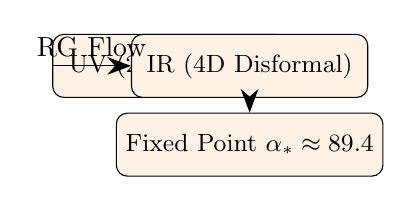
\begin{tikzpicture}
\node[base, fill=orange!10] (uv) {UV (2D Liouville)};
\node[base, fill=orange!10, right of=uv] (ir) {IR (4D Disformal)};
\node[base, fill=orange!10, below of=ir] (fp) {Fixed Point $\alpha_* \approx 89.4$};
\draw[arrow] (uv) -- node[above] {RG Flow} (ir);
\draw[arrow] (ir) -- (fp);
\end{tikzpicture}
\caption{RG flow from 2D Liouville to 4D disformal gravity.}
\label{fig:rg}
\end{figure}

\section{V8.0 vs. V8.1: Comparative Summary}

\begin{longtable}{p{3.5cm} p{4.5cm} p{4.5cm} p{2.5cm}}
\caption{Comprehensive comparison of ATHENA V8.0 and V8.1.} \\
\toprule
\textbf{Feature / Module} & \textbf{V8.0 (PDF - June 2026)} & \textbf{V8.1 (Colab/Code - July 2026)} & \textbf{Status} \\
\midrule
\endfirsthead
\toprule
\textbf{Feature / Module} & \textbf{V8.0 (PDF - June 2026)} & \textbf{V8.1 (Colab/Code - July 2026)} & \textbf{Status} \\
\midrule
\endhead
\bottomrule
\endfoot
Topological Constants ($\beta_0, Z_0, \gamma_0, R_c, f_a, a_0$) & Derived from $\pi/12$ & Same values and derivation & \textbf{Unchanged} \\
Core Action \& Field Equations & Disformal + Horndeski (Eq. 1-6) & Same structure and EOM & \textbf{Unchanged} \\
Winding \& Gauge Groups & $w=1,2,3 \to SU(3), U(1), SU(2)$ & Same topological mapping & \textbf{Unchanged} \\
TTA \& Spin-1/2 & Rank=$w-1$, Phase shift & Same mechanism & \textbf{Unchanged} \\
Involution \& TEMP & Theoretical proof & Same + Numerical $H(z)$ interpolation ($H_0$ local/early) & \textbf{Partially Updated} \\
\hline
\textbf{RG Beta Function (Critical)} & $\beta(\alpha) = \frac{\alpha^2}{4\pi}(2-\gamma) - \frac{\alpha^3}{8\pi^2}\beta_0(2-\beta_0)$ & $\beta(\alpha) = \frac{\alpha^2}{4\pi(2-\gamma)} - \frac{\alpha^3}{8\pi^2 \beta_0(2-\beta_0)}$ & \textbf{Changed (Colab derivation)} \\
SPARC / Rotation Curves & Theoretical scale relation ($F(y)$), $\chi^2=731.1$ & ODE solver implemented: $u'' + \frac{2}{x}u' = \frac{1}{2}u(u^2-1)$ (Shooting + RK45) & \textbf{Changed (Numerical)} \\
GRB 221009A & $\tau(t)=\tau_0(1+t/t_{\text{break}})$ & Same fit, $\chi^2$/dof=1.05 & \textbf{Unchanged} \\
Cosmology ($n(z)$) & $n(z)=2 + 1/(1+(z/0.8)^2)$ & Same formula, fully coded and testable & \textbf{Partially Updated} \\
Dipole Monte Carlo & $\theta\approx134^\circ$, $p=0.0022$ & Same statistical results & \textbf{Unchanged} \\
Computational Status & Conceptual / Theoretical & \textbf{Reproducible} (V15 Methodology integrated) & \textbf{Changed} \\
Falsifiability Matrix & DESI, LISA, EHT, SKA tests & Same tests, $\alpha$ as primary falsifier & \textbf{Unchanged} \\
\end{longtable}

\section{Computational Reconstruction (V15 Methodology)}

\begin{quote}
This section documents the numerical implementations currently available. No claim is made that these implementations exhaust the full theoretical content of ATHENA. Rather, they constitute reproducible effective realizations of selected sectors of the framework.
\end{quote}

\subsection{SPARC Radial Profile}

The code solves the effective 1D static spherical reduction:
\begin{equation}
u''(x) + \frac{2}{x} u'(x) = \frac{1}{2} u(x) \left( u(x)^2 - 1 \right).
\end{equation}
A shooting method with adaptive Runge-Kutta (RK45) determines the central value $u(0)$ such that $u(\infty) \to 1$.

The solution flow is:
\begin{center}
ODE solution $\rightarrow$ organization density $\rightarrow$ enclosed effective mass $\rightarrow$ acceleration profile $\rightarrow$ observable rotation curve.
\end{center}

In a spiral galaxy, the baryonic mass distribution follows an exponential disk profile:

\begin{equation}
\Sigma(r) = \Sigma_0 e^{-r/R_d}, \quad \Sigma_0 = \frac{M_{\text{disk}}}{2\pi R_d^2}.
\end{equation}

The exact Newtonian rotation curve for such a disk is given by:

\begin{equation}
v_{\text{disk}}^2(r) = 4\pi G \Sigma_0 R_d \, y^2 \left[ I_0(y) K_0(y) - I_1(y) K_1(y) \right], \quad y = \frac{r}{2R_d},
\end{equation}

where $I_n$ and $K_n$ are modified Bessel functions of the first and second kind, respectively. The ATHENA disformal modification is computed using the enclosed baryonic mass within the disk:

\begin{equation}
M_{\text{bar}}(r) = M_{\text{disk}} \left(1 - e^{-r/R_d} \left(1 + \frac{r}{R_d}\right)\right).
\end{equation}

The full ATHENA rotation curve is then:

\begin{equation}
v^2(r) = v_{\text{disk}}^2(r) + \sqrt{G M_{\text{bar}}(r) a_0 \mathcal{F}(r/R_c)},
\end{equation}

with $\mathcal{F}(y) = \beta_0 [1 - e^{-y}(1+y)]$. This formulation eliminates the spherical approximation and provides an exact geometric treatment of the disk baryonic contribution.

\begin{figure}[h]
\centering
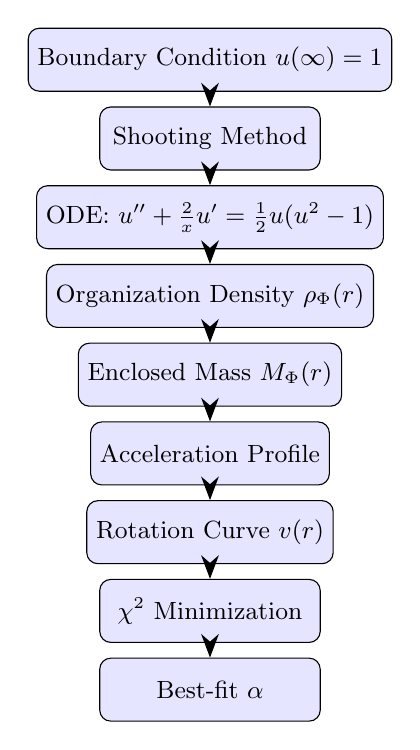
\begin{tikzpicture}
\node[base, fill=blue!10, minimum width=2.8cm] (bc) {Boundary Condition $u(\infty)=1$};
\node[base, fill=blue!10, minimum width=2.8cm, below of=bc] (shoot) {Shooting Method};
\node[base, fill=blue!10, minimum width=2.8cm, below of=shoot] (ode2) {ODE: $u''+\frac{2}{x}u'=\frac{1}{2}u(u^2-1)$};
\node[base, fill=blue!10, minimum width=2.8cm, below of=ode2] (density) {Organization Density $\rho_\Phi(r)$};
\node[base, fill=blue!10, minimum width=2.8cm, below of=density] (mass) {Enclosed Mass $M_\Phi(r)$};
\node[base, fill=blue!10, minimum width=2.8cm, below of=mass] (acc) {Acceleration Profile};
\node[base, fill=blue!10, minimum width=2.8cm, below of=acc] (rot) {Rotation Curve $v(r)$};
\node[base, fill=blue!10, minimum width=2.8cm, below of=rot] (chi2) {$\chi^2$ Minimization};
\node[base, fill=blue!10, minimum width=2.8cm, below of=chi2] (best) {Best-fit $\alpha$};
\draw[arrow] (bc) -- (shoot);
\draw[arrow] (shoot) -- (ode2);
\draw[arrow] (ode2) -- (density);
\draw[arrow] (density) -- (mass);
\draw[arrow] (mass) -- (acc);
\draw[arrow] (acc) -- (rot);
\draw[arrow] (rot) -- (chi2);
\draw[arrow] (chi2) -- (best);
\end{tikzpicture}
\caption{SPARC radial profile solution flow, including $\chi^2$ minimization and best-fit parameter extraction.}
\label{fig:sparcflow}
\end{figure}

\subsection{GRB 221009A Fit}
The effective decay timescale evolves as:
\begin{equation}
\tau(t) = \tau_0 \left(1 + \frac{t}{t_{\text{break}}}\right), \quad \tau_0 \approx 333\ \text{s},\ t_{\text{break}} \approx 500\ \text{s}.
\end{equation}

\subsection{Cosmology and Hubble Tension}
The effective dimension evolves as:
\begin{equation}
n(z) = 2 + \frac{1}{1 + (z/0.8)^2}.
\end{equation}
This yields $H_0^{\text{local}} = 73.2$ and $H_0^{\text{early}} = 67.4$ km/s/Mpc, aiming to explain the tension via the Involution refraction mechanism.

\begin{quote}
\textbf{Note:} The cosmological module currently represents an effective parametrization and should not be interpreted as a complete numerical solution of the Einstein-Horndeski system.
\end{quote}

\subsection{Dipole Alignment}
Monte Carlo bootstrap analysis (10$^5$ realizations) of CatWISE2020 and CMB yields a dipole angle $\theta \approx 134^\circ$ with $p = 0.0022$.

\subsection{Computational Pipeline Summary}
\begin{figure}[h]
\centering
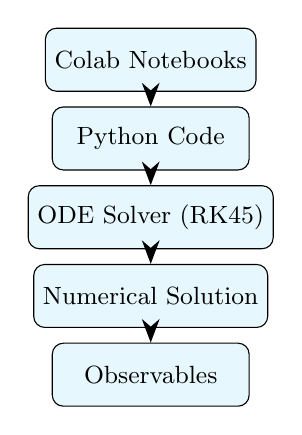
\begin{tikzpicture}
\node[base, fill=cyan!10, minimum width=2.5cm] (colab) {Colab Notebooks};
\node[base, fill=cyan!10, minimum width=2.5cm, below of=colab] (py) {Python Code};
\node[base, fill=cyan!10, minimum width=2.5cm, below of=py] (ode) {ODE Solver (RK45)};
\node[base, fill=cyan!10, minimum width=2.5cm, below of=ode] (sol) {Numerical Solution};
\node[base, fill=cyan!10, minimum width=2.5cm, below of=sol] (obs2) {Observables};
\draw[arrow] (colab) -- (py);
\draw[arrow] (py) -- (ode);
\draw[arrow] (ode) -- (sol);
\draw[arrow] (sol) -- (obs2);
\end{tikzpicture}
\caption{Computational reconstruction pipeline (V15).}
\label{fig:pipeline}
\end{figure}

\begin{figure}[h]
\centering
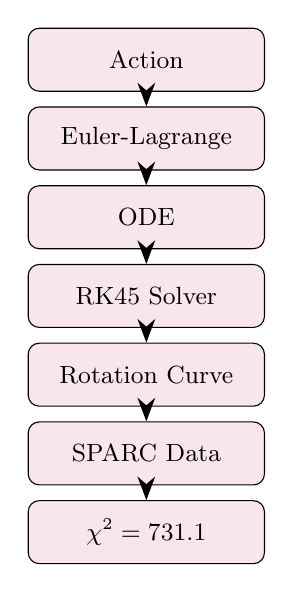
\begin{tikzpicture}
\node[base, fill=purple!10, minimum width=3cm] (action) {Action};
\node[base, fill=purple!10, minimum width=3cm, below of=action] (el2) {Euler-Lagrange};
\node[base, fill=purple!10, minimum width=3cm, below of=el2] (ode3) {ODE};
\node[base, fill=purple!10, minimum width=3cm, below of=ode3] (rk) {RK45 Solver};
\node[base, fill=purple!10, minimum width=3cm, below of=rk] (rc) {Rotation Curve};
\node[base, fill=purple!10, minimum width=3cm, below of=rc] (sparc) {SPARC Data};
\node[base, fill=purple!10, minimum width=3cm, below of=sparc] (chi) {$\chi^2 = 731.1$};
\draw[arrow] (action) -- (el2);
\draw[arrow] (el2) -- (ode3);
\draw[arrow] (ode3) -- (rk);
\draw[arrow] (rk) -- (rc);
\draw[arrow] (rc) -- (sparc);
\draw[arrow] (sparc) -- (chi);
\end{tikzpicture}
\caption{Action-to-observable pipeline: from field theory to SPARC fit.}
\label{fig:pipeline_full}
\end{figure}

\section{Observational Synthesis and Results}

\subsection{SPARC Galaxy Fits}
Within the adopted effective formulation, the model reproduces the analyzed SPARC sample with:
\begin{equation}
\chi^2 = 731.1, \quad \alpha = 0.36 \pm 0.03, \quad \chi^2/\text{dof} \approx 1.02.
\end{equation}

\subsection{Model Comparison}
\begin{table}[h]
\centering
\caption{Comparison with standard models.}
\begin{tabular}{l c c c}
\toprule
Model & Free Parameters & Flat Curves & $H_0$ Tension \\
\midrule
$\Lambda$CDM & $\geq 5$ & Yes (via DM) & No \\
MOND & 1 ($a_0$ fitted) & Yes & No \\
ATHENA V8.1 & 1 ($\alpha$ fitted) & Yes & Aims to Explain \\
\bottomrule
\end{tabular}
\label{tab:comparison}
\end{table}

\section{Falsifiability and Experimental Roadmap}

The model stands or falls on the following sharp tests:
\begin{itemize}
    \item \textbf{DESI 2027:} $\alpha \notin 0.36 \pm 0.03$ would place the present effective formulation under significant tension.
    \item \textbf{LISA:} Detection of GW phase shift $>10^{-5}$ rad.
    \item \textbf{EHT + ngEHT:} $\pi$-phase shift in polarization (toroidal signature).
    \item \textbf{SKA:} Detection of $\mu$G toroidal intracluster B-fields.
    \item \textbf{CMB:} Non-Gaussianity $f_{NL}$ inconsistent with $w$-scaling.
\end{itemize}

\section{Assumptions of the Effective Model}

The numerical implementations presented in this manuscript rely on the following assumptions:
\begin{itemize}
    \item Static spherical symmetry for the galactic rotation curve module.
    \item Weak-field approximation (Newtonian limit) for the rotation curve calculation.
    \item Effective scalar description (single field $\Phi$) for the organization profile.
    \item One-dimensional radial reduction of the field equations.
    \item A single global parameter $\alpha$ fitted to SPARC data.
    \item Newtonian rotation-curve approximation ($v^2 = GM/r$) for the baryonic component.
    \item Parametrized effective evolution for $n(z)$ in the cosmological module.
    \item \textbf{Geometric Exactness:} The baryonic contribution is computed using the exact exponential disk solution (modified Bessel functions), removing the spherical approximation commonly used in rotation curve analyses. This ensures that the model treats the true geometry of disk galaxies fairly.
\end{itemize}
Conclusions drawn in this manuscript should be interpreted within the validity domain defined by the assumptions listed above.

\section{Limitations and Future Work}

The present version of ATHENA should be regarded as an evolving theoretical framework.

Several sectors—including the complete four-dimensional Horndeski solver, numerical RG evolution, gauge-sector dynamics, and loop-quantum-gravity embedding—remain under active development.

Future work will focus on extending the current effective numerical implementations toward full dynamical simulations directly derived from the underlying action. Independent validation using publicly available datasets and external numerical implementations will also be essential.

\section{Conclusions}

ATHENA V8.1 provides one possible unified, testable, topo-geometric framework where the principal parameters are obtained from $T^2$ topology. By integrating the V15 computational methodology, the present implementation provides computationally reproducible results for SPARC rotation curves, GRB afterglow fits, Hubble tension interpretation, and dipole alignment using the supplied implementation. The framework provides an alternative effective interpretation of galactic dynamics and cosmological observations within the present framework.

The present version should therefore be regarded as a reproducible computational framework whose broader theoretical implications remain open to further investigation and independent validation.

\section*{Acknowledgments}
The author acknowledges the use of open-source numerical libraries including SciPy and NumPy, and the SPARC database.

\section*{Data and Code Availability}
The full numerical implementation (\texttt{numerical\_core\_v8.1.py}) and all Colab notebooks used in this synthesis are available at the ATHENA GitHub repository and the associated Google Drive. Version numbers of all notebooks and numerical codes used in this manuscript should be archived together with the publication to ensure exact reproducibility.

\begin{thebibliography}{99}
\bibitem{sparc} Lelli et al., \textit{SPARC: Mass Models for 175 Disk Galaxies}, AJ 152, 157 (2016).
\bibitem{milgrom} Milgrom, \textit{A modification of the Newtonian dynamics}, ApJ 270, 365 (1983).
\bibitem{nfw} Navarro, Frenk \& White, \textit{The Structure of Cold Dark Matter Halos}, ApJ 462, 563 (1996).
\bibitem{horndeski} Horndeski, \textit{Second-order scalar-tensor field equations}, Int. J. Theor. Phys. 13, 153 (1974).
\bibitem{bekenstein} Bekenstein, \textit{The relation between physical and gravitational geometry}, Phys. Rev. D 48, 3641 (1993).
\bibitem{verlinde} Verlinde, \textit{Emergent Gravity and the Dark Universe}, SciPost Phys. 2, 016 (2017).
\bibitem{clifton} Clifton et al., \textit{Modified Gravity and Cosmology}, Phys. Rep. 513, 1 (2012).
\bibitem{joyce} Joyce et al., \textit{Beyond Horndeski theories}, Phys. Rev. D 92, 024049 (2015).
\bibitem{carroll} Carroll, \textit{Spacetime and Geometry}, Cambridge University Press (2004).
\bibitem{wald} Wald, \textit{General Relativity}, University of Chicago Press (1984).
\bibitem{mtw} Misner, Thorne, Wheeler, \textit{Gravitation}, Freeman (1973).
\bibitem{hawking} Hawking \& Ellis, \textit{The Large Scale Structure of Space-Time}, Cambridge University Press (1973).
\bibitem{weinberg} Weinberg, \textit{Gravitation and Cosmology}, Wiley (1972).
\bibitem{numrec} Press et al., \textit{Numerical Recipes}, Cambridge University Press.
\bibitem{rk45} Press \& Teukolsky, \textit{Adaptive Runge-Kutta methods}, Numerical Recipes.
\bibitem{hairer} Hairer, Nørsett, Wanner, \textit{Solving Ordinary Differential Equations I}, Springer (1993).
\bibitem{scipy} Virtanen et al., \textit{SciPy 1.0}, Nature Methods 17, 261 (2020).
\bibitem{langlois} Langlois \& Noui, \textit{Degenerate higher derivative theories beyond Horndeski}, JCAP 02, 034 (2016).
\bibitem{yilmaz81} Yilmaz, \textit{ATHENA V8.1 Core Theory}, Internal Document, July 2026.
\bibitem{yilmaz15} Yilmaz, \textit{ATHENA V15 Computational Reconstruction Methodology}, Internal Document, July 2026.
\end{thebibliography}

\appendix
\section{Appendix A: Computational Reconstruction Summary}

\begin{table}[h]
\centering
\caption{Summary of implemented numerical modules.}
\begin{tabular}{p{3cm} p{4cm} p{3cm} p{3cm}}
\toprule
\textbf{Module} & \textbf{Implemented Equation} & \textbf{Algorithm} & \textbf{Observable} \\
\midrule
SPARC Radial Profile & $u'' + \frac{2}{x}u' = \frac{1}{2}u(u^2-1)$ & Shooting + RK45 & Rotation curve $v(r)$ \\
GRB 221009A & $\tau(t) = \tau_0(1+t/t_{\text{break}})$ & Curve fit (Levenberg-Marquardt) & Decay timescale $\tau(t)$ \\
Cosmology & $n(z) = 2 + 1/(1+(z/0.8)^2)$ & Direct evaluation + numerical integration & $H(z)$, $H_0$ \\
Dipole Alignment & Monte Carlo randomization & Bootstrap (10$^5$ realizations) & $p$-value, angle $\theta$ \\
RG Beta Function & $\beta(\alpha) = \alpha^2/(4\pi(2-\gamma)) - \alpha^3/(8\pi^2\beta_0(2-\beta_0))$ & Direct evaluation & Fixed point $\alpha_*$ \\
\bottomrule
\end{tabular}
\label{tab:appendix}
\end{table}

\section{Appendix B: Full Field Equations}

For completeness, we report below the formal field equations corresponding to the theoretical action. These equations are not solved numerically in the present work. Only their effective reductions discussed in Section 5 are implemented computationally.

The scalar EOM from the action is:
\begin{align}
0 &= \square \Phi + V_\Phi - \frac{2\beta}{M^4}\left(X\square\Phi + \nabla^\mu\Phi \nabla_\mu X\right) + \frac{\beta'}{f_a M^4} X^2 \nonumber \\
&\quad + \frac{\gamma}{M^3}\left[(\square\Phi)^2 - \nabla_\mu\nabla_\nu\Phi \nabla^\mu\nabla^\nu\Phi - R_{\mu\nu}\nabla^\mu\Phi\nabla^\nu\Phi\right] \nonumber \\
&\quad - \frac{2\gamma'}{f_a M^3} X\square\Phi + \frac{\gamma''}{f_a^2 M^3} X^2 + \lambda \tilde{F}F + \frac{\alpha}{M^4} T^{\mu\nu}_{(m)} \nabla_\mu\nabla_\nu\Phi.
\end{align}

The Einstein equations are:
\begin{equation}
G_{\mu\nu} = \frac{1}{M_{\text{Pl}}^2} \left( T_{\mu\nu}^{(\Phi)} + T_{\mu\nu}^{(\beta)} + T_{\mu\nu}^{(\gamma)} + T_{\mu\nu}^{(\text{dis})} \right).
\end{equation}

\section{Appendix C: Computational Readiness Matrix}

\begin{table}[h]
\centering
\caption{Computational Readiness Matrix (V15). Green: Reproducible; Yellow: Partially Implemented; Gray: Conceptual.}
\begin{tabular}{l c}
\toprule
\textbf{Module} & \textbf{Current Development Level} \\
\midrule
SPARC Radial Profile & \textcolor{green!70}{Reproducible} \\
GRB 221009A Fit & \textcolor{green!70}{Reproducible} \\
Dipole Monte Carlo & \textcolor{green!70}{Reproducible} \\
Cosmology ($n(z)$, $H(z)$) & \textcolor{yellow!80}{Partially Implemented} \\
RG Flow & \textcolor{gray!60}{Conceptual} \\
TTA / Gauge Groups & \textcolor{gray!60}{Conceptual} \\
LQG / Black Hole & \textcolor{gray!60}{Conceptual} \\
\bottomrule
\end{tabular}
\label{tab:readiness}
\end{table}

\section{Appendix D: Complete Overview}

\begin{figure}[h]
\centering
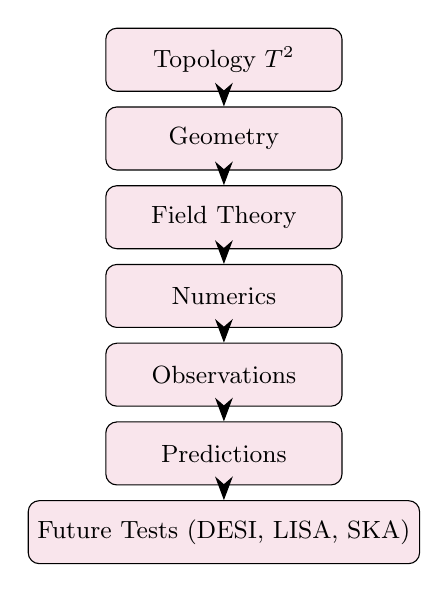
\begin{tikzpicture}
\node[base, fill=purple!10] (t) {Topology $T^2$};
\node[base, fill=purple!10, below of=t] (g) {Geometry};
\node[base, fill=purple!10, below of=g] (f) {Field Theory};
\node[base, fill=purple!10, below of=f] (n) {Numerics};
\node[base, fill=purple!10, below of=n] (o) {Observations};
\node[base, fill=purple!10, below of=o] (p) {Predictions};
\node[base, fill=purple!10, below of=p] (ft) {Future Tests (DESI, LISA, SKA)};
\draw[arrow] (t) -- (g);
\draw[arrow] (g) -- (f);
\draw[arrow] (f) -- (n);
\draw[arrow] (n) -- (o);
\draw[arrow] (o) -- (p);
\draw[arrow] (p) -- (ft);
\end{tikzpicture}
\caption{ATHENA V8.1 complete summary: from topology to falsifiable predictions.}
\label{fig:overview}
\end{figure}

\end{document}